%%% In this section, you will describe all of the various artifacts that you will generate and maintain during the project life cycle. Describe the purpose of each item below, how the content will be generated, where it will be stored, how often it will be updated, etc. Replace the default text for each section with your own description. Reword this paragraph as appropriate.

\subsection{Major Documentation Deliverables}

\subsubsection{Project Charter}
The Project charter is being maintained at a weekly basis. Our team meets at least once a week, every week. The designated meeting date is every Friday, but if more times needs to be allocated to the project then we may meet again. The initial version of the project charter will be delivered on October 1, 2018. The final version of the project charter will be delivered sometime in May 2019.

\subsubsection{System Requirements Specification}
The System Requirements Specification Documentation will be maintained at our weekly meeting. The team meeting for this specific document will only occur during it's designated sprint (Sprint 2). The SRS documentation will be updated under the circumstance of a system requirement being inadequately defined. The initial version will be delivered on October 23, 2018. The final version of the SRS documentation will be delivered sometime in May 2019.

\subsubsection{Architectural Design Specification}
The Architectural Design Specification Documentation will be maintained at our weekly meeting. The team meeting for this specific document will only occur during it's designated sprint (Sprint 3). If our team discovers faults in our design patterns, then we may have to update the architectural design specifications. The initial version will be delivered on November 13, 2018. The final version of the ADS documentation will be delivered sometime in May 2019.

\subsubsection{Detailed Design Specification}
The Architectural Design Specification Documentation will be maintained at our weekly meeting. The team meeting for this specific document will only occur during it's designated sprint (Sprint 4). If our team creates unique Jenga blocks, then we will have to update our DDS documentation with the correct drawings and dimensions of the blocks. The initial version will be delivered on December 04, 2018. The final version of the DDS documentation will be delivered sometime in May 2019.

\subsection{Recurring Sprint Items}

\subsubsection{Product Backlog}
Items will be added to our backlog when the SRS documentation is changed to specify new requirements. The backlog for this project is being shared with the collaborative platform Google Drive, using Google Sheets. Items in the backlog are being prioritized by team votes during our weekly meetings.

\subsubsection{Sprint Planning}
Each sprint is planned and documented during our team meetings. Using a sprint backlog chart, we can maintain and split the required work for a given sprint fairly between each team member. During SD1 there are 4 sprints, each being two weeks in length. 

\subsubsection{Sprint Goal}
Our team as a whole discusses and decides the sprint goal together. Our customer's, Dr. McMurrough, involvement was giving our team a project with the UR5 Robot Arm. Other than this involvement, our team decides the sprint goal.

\subsubsection{Sprint Backlog}
The product backlog items that make their way into the sprint backlog are decided as a team during our weekly team meetings. The backlog is currently maintained with the collaborative platform Google Drive, using Google sheets and Microsoft Excel.  

\subsubsection{Task Breakdown}
Individual tasks from the sprint backlog are assigned to a team member based on a combination of team decisions and voluntarily claim of the tasks. Time on each task are documented by the expected hours it will take and the actual hours the task took to complete. The sprint backlog is located in our teams Google Drive as a Google Sheets file.

\subsubsection{Sprint Burn Down Charts}
Our team as a whole is responsible for keeping up with, and maintaining, the burn down chart during each sprint. The burn down charts allows us to input the amount of time allocated to a task during a sprint, so that it will then automatically update the burn down chart. Doing this allows our team to view the progress made on the project during a given sprint. The burn down chart is located in our teams Google Drive as a Google Sheets file. (Refer to Figure 3)

\begin{figure}[ht]
    \centering
    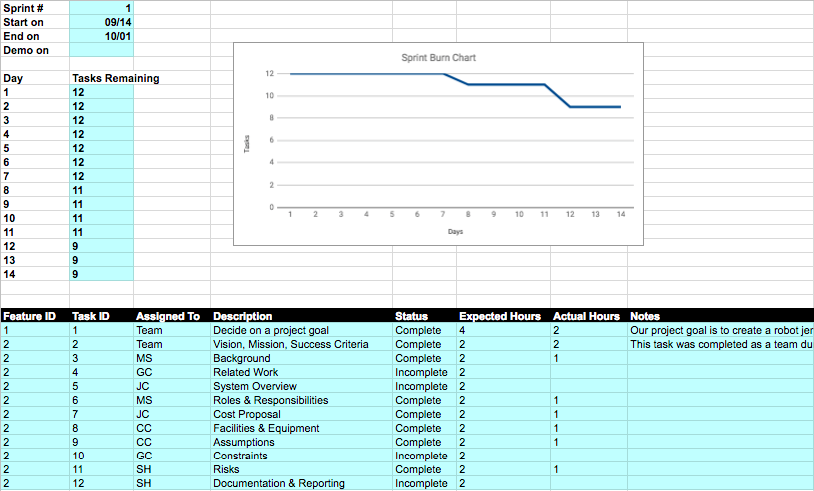
\includegraphics[width=1.0\textwidth]{images/sprint_burndown.png}
    \caption{Sprint burndown chart for Sprint 1}
\end{figure}

\subsubsection{Sprint Retrospective}
We will meet during the week between sprints and document in our engineering notebooks how the sprint went overall. We can also discuss what what we need to do better as a team.

\subsubsection{Individual Status Reports}
The individual status report will be completed every sprint week and discussed quickly at the weekly team meeting. We can fill out the individual status report in our engineering notebooks so we will have a record to improve upon.

\subsubsection{Engineering Notebooks}
We will fill out our individual status reports as well as any technical progress we have made in the engineering notebook. For accountability we will discuss our individual status reports at our weekly sprint meeting. We will also be able to sign the notebooks as witnesses during those weekly meetings as well.

\subsection{Closeout Materials}

\subsubsection{System Prototype}
Our system prototype will be to have a robot that will be able to scan the tower and play the game in favorable conditions for the robot. The robot will hopefully be able to get out of the lab and be demonstrated off-site. If we were to take it off-site to a conference which is the ultimate goal we need to make sure that it can handle playing against a human who doesn't know how the robot works.

\subsubsection{Project Poster}
Our project poser will be a 36" by 48" poster board that we will deliver near the final sprint to outline some of the features and development of our project. We may also have the robot out for an in-person demonstration.

\subsubsection{Web Page}
We intend to develop a simple webpage that states what our robot is capable of doing, who is on our team, the Doxygen documentation that we develop, and a link to Cloud9 Perception.

\subsubsection{Demo Video}
We will make a demo video displaying at least a part of a game that the robot will play. We will also produce plenty of B-roll footage throughout the semester that we can also upload and share to show the progress of the robot development.

\subsubsection{Source Code}
The source code will be maintained under a GitHub organization at https://github.com/jovialmcnulty. We will be adopting Git version control, in which the full source code of the project will be provided to the customer. We will be using a GNU 

\subsubsection{Source Code Documentation}
Code documentation will be done during code creation or as soon as possible after code creation. We will use Doxygen to generate our source code documentation, allowing us to provide that documentation in a browsable HTML file. 

%\subsubsection{Hardware Schematics}

\subsubsection{CAD files}
We will be designing our own set of Jenga blocks to be used by the UR5 Jenga playing robot. These blocks will be designed by our team and 3D printed. We will use Tinkercad to generate the model for an individual block. The model will be saved as an STL file. We will be using Cura to generate slices for the models, providing printable G-code.

\subsubsection{Installation Scripts}
We will provide a catkin package so the client can easily install the robot controls onto their own UR5 robot through ROS. The catkin package will include all dependencies for the robot setup, including drivers for the camera and gripper.

We will also include an installation script for the computer vision and user interface portions. These components will be installed using our installation script, and run on a PC that is working behind the scenes and providing vision and some control data to the robot.

\subsubsection{User Manual}
The UR5 Jenga playing robot will include a digital setup manual created using LaTeX. The setup manual will include instructions on how to setup the initial game state and game space markers. The manual will also describe how to calibrate the robot arm within the game space, and how to operate the user interface that controls when the robot takes its turn.

We will also include physical manuals that describe the rules for the game of Jenga, and how to play the game with the UR5 Jenga playing robot arm as your competitor. These physical copies of instructions are meant to be handouts used as part of the display, so that users interacting with the display will know the rules of the game.
